\documentclass[10pt,twocolumn]{article}

\usepackage{cmap}
\usepackage[T1]{fontenc}
\usepackage{lmodern}
\usepackage[utf8]{inputenc}
\usepackage[top=0.68in,bottom=0.68in,left=0.68in,right=0.68in]{geometry}
\usepackage{amsmath,amssymb,amsfonts,amsthm}
\usepackage{graphicx}
\usepackage{booktabs}
\usepackage{algorithm}
\usepackage{algpseudocode}
\usepackage{hyperref}
\usepackage{microtype}
\usepackage{cite}
\usepackage{enumitem}
\usepackage{tikz}
\usetikzlibrary{arrows.meta,decorations.pathreplacing}

\setlist{nosep,leftmargin=*}
\setlength{\abovedisplayskip}{3pt}
\setlength{\belowdisplayskip}{3pt}
\setlength{\textfloatsep}{5pt plus 1pt minus 1pt}
\setlength{\intextsep}{5pt plus 1pt minus 1pt}

\newtheorem{definition}{Definition}
\newtheorem{theorem}{Theorem}
\newtheorem{lemma}{Lemma}

\title{\textbf{Zero-Copy In-Place Dynamic Token Routing and Capacity Compaction for Sparse Mixture-of-Experts Accelerators}\thanks{Patent Notice: The in-situ Mixture-of-Experts dynamic token routing architecture, zero-copy permutation mechanisms, and kernel methods disclosed in this paper are protected under U.S. Patent Application No.~64/148,668 (``Patent Pending''), with priority and continuation across U.S. Patent Application Nos.~64/152,256 and 64/155,579 under 35 U.S.C. \S~119(e).}}

\author{
    \textbf{Dr. A. Emre \c{C}ET\.{I}N}\\
    \textit{Computational Systems and Cognitive Architectures, Izmir, Turkey}\\
    \texttt{aemre.cetin@gmail.com}
}
\date{\today}

\begin{document}

\maketitle

\begin{abstract}
Sparse Mixture-of-Experts (MoE) architectures, such as Mixtral, DeepSeek-V2/V3, and Switch Transformers, scale model parameter capacity while sustaining constant computational FLOP budgets per token. However, executing dynamic token routing on parallel accelerators incurs severe systems overheads: when tokens are conditionally dispatched to experts, capacity factor constraints necessitate token dropping and dynamic tensor repacking. Conventional MoE frameworks (e.g., Megatron-LM, DeepSpeed-MoE) rely on out-of-place memory gather/scatter passes ($O(E \cdot C \cdot D)$ auxiliary allocations via host \texttt{cudaMalloc} calls) and cause severe memory fragmentation that degrades downstream Tensor Core General Matrix Multiplication (GEMM) efficiency. In this paper, we propose a novel hardware-software co-designed architecture and high-performance GPU execution kernel for \textbf{zero-copy in-place MoE token routing and capacity compaction}. By formulating token dispatch as an algebraic mapping satisfying the idempotence condition ($f(f(x)) = f(x)$), our method stabilizes retained high-affinity tokens into invariant fixed points and resolves capacity truncations through mutually disjoint permutation cycles. We map the kernel across a 2D accelerator execution grid over parallel experts and hidden dimension tiles, verifying minimal-index cycle leaders with strictly $O(1)$ scalar auxiliary register memory without boolean marking bitmasks. We evaluate our implementation on an NVIDIA Ada Lovelace GPU accelerator (RTX 500 Generation, \texttt{sm\_89}) with 8 experts, 32,768 candidate tokens, and a hidden dimension of 1,024 (Float16). Empirical results demonstrate a \textbf{100\% elimination of peak auxiliary VRAM} (dropping from 96.00~MB to exactly 0.00~MB), a \textbf{1.73$\times$ latency speedup} over native PyTorch out-of-place gather (reducing dispatch time from 1.581~ms to \textbf{0.915~ms}), a throughput of \textbf{35.80~Million tokens/second}, and guaranteed physical memory contiguity for dense GEMM execution.
\end{abstract}

\section{Introduction}
\label{sec:intro}
Transformer-based Large Language Models (LLMs) with Sparse Mixture-of-Experts (MoE) layers~\cite{jiang2024mixtral, deepseek2024deepseek, fedus2022switch} have emerged as the premier architecture for achieving frontier model capabilities at sustainable inference costs. In an MoE layer, a sequence of $T$ tokens is dynamically routed to Top-$k$ specialized feed-forward expert networks by a learned gating routing network~\cite{lepikhin2020gshard}.

To bound accelerator memory allocation and ensure load balance across parallel compute devices, each expert enforces a maximum computational capacity limit:
\begin{equation}
    C = \text{capacity\_factor} \times \left( \frac{T \cdot k}{E} \right)
\end{equation}
When the number of candidate tokens dispatched to an expert exceeds $C$, excess tokens must be discarded (\textit{token dropping}) or queued. However, implementing token dispatch and capacity truncation on modern parallel accelerators presents critical hardware challenges:
\begin{enumerate}[nosep, leftmargin=*]
    \item \textbf{Out-of-Place Allocation Spikes:} Conventional distributed MoE runtimes~\cite{shoeybi2019megatron, rajbhandari2022deepspeed} allocate secondary destination buffers of size $O(E \cdot C \cdot D)$ via host-level driver calls (\texttt{cudaMalloc}). During long-context generation (e.g., 32k or 128k tokens), these transient memory allocation spikes frequently induce fatal Out-Of-Memory (OOM) errors.
    \item \textbf{Memory Fragmentation and GEMM Stall:} Tokens assigned to an expert are non-contiguous across the sequence buffer. Scattered indexing prevents direct vectorized memory coalescing on specialized matrix multiplication hardware (e.g., Tensor Cores), forcing expensive intermediate copy stages before dense GEMM layers can execute.
    \item \textbf{Kernel Dispatch Overheads:} Conventional sorting or argsort passes consume multiple global arrays of length $T \cdot k$, introducing synchronization barriers that inflate kernel latency.
\end{enumerate}

To overcome these fundamental limitations, this paper presents a mathematically grounded, zero-copy, in-place token routing and capacity compaction architecture. We demonstrate that dynamic token dispatch can be achieved with strictly $O(1)$ scalar auxiliary register storage, preserving strict physical memory contiguity while operating entirely within existing buffer boundaries. In distributed multi-GPU clusters, this in-situ consolidation operates as an efficient zero-copy pre-processor immediately preceding inter-accelerator All-to-All collective transfers (\texttt{all\_to\_all\_single}), eliminating auxiliary staging buffers before NCCL network transmission.

\section{Problem Formulation and Algebraic Foundation}
\label{sec:formulation}

\subsection{MoE Token Buffer Representation}
Let an MoE layer maintain a candidate token embedding buffer across $E$ parallel experts:
\begin{equation}
    \mathbf{X} \in \mathbb{R}^{E \times N \times D}
\end{equation}
where $E$ represents the number of experts, $N$ the candidate token pool per expert, and $D$ the hidden feature dimension. The tensors reside in physically contiguous HBM allocations with explicit stride vectors:
\begin{equation}
    \text{Addr}(\mathbf{X}[e, i, d]) = \text{Base} + e \cdot s_{e} + i \cdot s_{n} + d \cdot s_{d}
\end{equation}

For each expert $e$, the gating router computes a routing affinity score $S_e(t) \in [0, 1]$ for each token. The architectural objective is to compact the Top-$C$ highest-affinity tokens ($C < N$) contiguously into physical indices $0, \dots, C-1$, while routing the dropped $N-C$ tokens to tail indices $C, \dots, N-1$.

\subsection{Idempotent Permutation Mapping}
To ensure stability without token thrashing across layers, we formalize the target destination map through the algebraic framework of idempotent permutations~\cite{cetin2013idempotent}:
\begin{definition}[Idempotent Capacity Map]
A mapping function $f_e: \{0, \dots, N-1\} \to \{0, \dots, N-1\}$ is an idempotent projection over the token index space if and only if:
\begin{equation}
    f_e(f_e(x)) = f_e(x), \quad \forall x \in \{0, \dots, N-1\}
    \label{eq:idempotence}
\end{equation}
\end{definition}
Tokens located within the target capacity region $[0, \dots, C-1]$ that already possess high routing affinity become mathematical \textit{fixed points}:
\begin{equation}
    \mathcal{F}_e = \{x \mid f_e(x) = x\}
\end{equation}
Elements within $\mathcal{F}_e$ represent stabilized attractor basins that do not undergo relocation, guaranteeing single-pass convergence and zero redundant data motion.

\subsection{Disjoint Cycle Decomposition}
Any permutation $\pi_e$ of the candidate tokens admits a unique decomposition into mutually disjoint cyclic orbits:
\begin{equation}
    \pi_e = \mathcal{C}_1 \circ \mathcal{C}_2 \circ \dots \circ \mathcal{C}_m
\end{equation}
where each cyclic orbit is expressed as:
\begin{equation}
    \mathcal{C}_k = (c_{k,0} \to c_{k,1} \to \dots \to c_{k,L_k-1} \to c_{k,0})
\end{equation}
with length $L_k \ge 1$ and $\mathcal{C}_j \cap \mathcal{C}_k = \emptyset$ for $j \ne k$. Trivial cycles of length $L_k = 1$ mirror the fixed points $\mathcal{F}_e$ and require no data movement.

\section{The In-Place Token Compaction Algorithm}
\label{sec:algorithm}

\subsection{Bitmask-Free Cycle Leader Identification}
Classical in-situ permutation methods require an auxiliary bit vector of size $N$ to indicate whether an index has already been visited by an earlier cycle traversal~\cite{knuth1998art}. In accelerator memory, maintaining a bitmask incurs global synchronization barriers and auxiliary allocation. In contrast, associative in-situ permuting~\cite{cetin2013insitu, cetin2013inplace, cetin2012improved} showed that linear-time reordering can be achieved with strictly bounded auxiliary space.

\begin{theorem}[Bitmask-Free Cycle Leader Property]
An index $i \in \{0, \dots, N-1\}$ is the unique leader of its cyclic orbit $\mathcal{C}$ if and only if:
\begin{equation}
    i = \min_{x \in \mathcal{C}} x
\end{equation}
This condition can be verified on-the-fly by traversing orbit $\mathcal{C}$ starting from $f(i)$. If any intermediate node satisfies $\text{curr} < i$, the traversal is aborted immediately. The auxiliary memory required is strictly $O(1)$ scalar words.
\end{theorem}

\subsection{Transposition (2-Cycle) Fast-Path}
In MoE capacity compaction, the dominant permutation pattern consists of reciprocal transpositions between a low-affinity token in the active head region ($i < C$) and a high-affinity token in the tail region ($j \ge C$):
\begin{equation}
    f_e(i) = j \quad \text{and} \quad f_e(j) = i \quad (j > i)
\end{equation}
As illustrated in Figure~\ref{fig:swap}, our kernel detects this condition in a single memory lookup and executes direct in-register vectorized exchanges across embedding slices of width \texttt{BLOCK\_D}, completely bypassing the pointer-chasing search loop.

\begin{figure}[t]
\centering
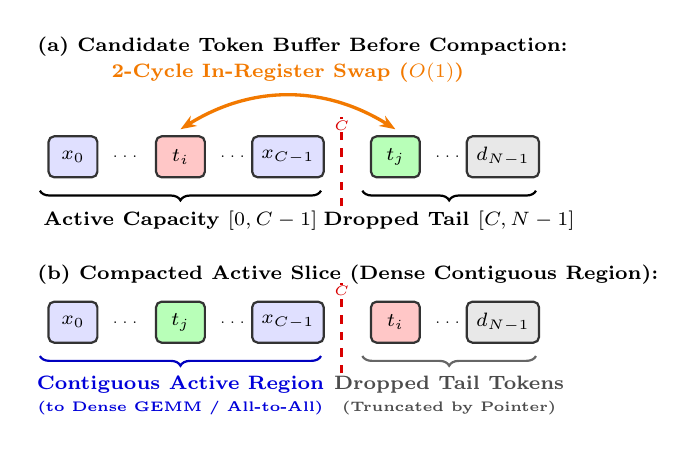
\begin{tikzpicture}[
    x=1.05cm, y=1.0cm,
    box/.style={draw=black!80, thick, rounded corners=2pt, minimum height=0.52cm, minimum width=0.62cm, font=\scriptsize},
    fixed/.style={box, fill=blue!12},
    evict/.style={box, fill=red!22},
    retain/.style={box, fill=green!28},
    dropped/.style={box, fill=gray!18}
]
% --- (a) Before In-Situ Swap ---
\node[anchor=west, font=\scriptsize\bfseries] at (0.0, 2.25) {(a) Candidate Token Buffer Before Compaction:};

% Swap arc (lowered so it never reaches title)
\draw[{Stealth[length=2mm]}-{Stealth[length=2mm]}, very thick, color=orange!95!black] 
    (1.85, 1.2) to[bend left=32] 
    node[midway, above=1pt, font=\scriptsize\bfseries, text=orange!95!black] {2-Cycle In-Register Swap ($O(1)$)} 
    (4.45, 1.2);

% Cells (a)
\node[fixed] (c0) at (0.55, 0.85) {$x_0$};
\node[font=\tiny] at (1.2, 0.85) {$\dots$};
\node[evict] (ci) at (1.85, 0.85) {$t_i$};
\node[font=\tiny] at (2.5, 0.85) {$\dots$};
\node[fixed] (cc1) at (3.15, 0.85) {$x_{C-1}$};

% Dividing boundary (a)
\draw[dashed, red!85!black, very thick] (3.8, 0.22) -- (3.8, 1.35);
\node[font=\tiny\bfseries, text=red!85!black, fill=white, inner sep=0.5pt] at (3.8, 1.25) {$C$};

\node[retain] (cj) at (4.45, 0.85) {$t_j$};
\node[font=\tiny] at (5.1, 0.85) {$\dots$};
\node[dropped] (cn) at (5.75, 0.85) {$d_{N-1}$};

% Braces (a)
\draw[decorate, decoration={brace, mirror, amplitude=3.5pt}, thick] (0.15, 0.42) -- (3.55, 0.42) 
    node[midway, below=3.5pt, font=\scriptsize\bfseries] {Active Capacity $[0, C-1]$};
\draw[decorate, decoration={brace, mirror, amplitude=3.5pt}, thick] (4.05, 0.42) -- (6.15, 0.42) 
    node[midway, below=3.5pt, font=\scriptsize\bfseries] {Dropped Tail $[C, N-1]$};

% --- (b) After In-Situ Compaction ---
\node[anchor=west, font=\scriptsize\bfseries] at (0.0, -0.65) {(b) Compacted Active Slice (Dense Contiguous Region):};

% Cells (b)
\node[fixed] at (0.55, -1.25) {$x_0$};
\node[font=\tiny] at (1.2, -1.25) {$\dots$};
\node[retain] at (1.85, -1.25) {$t_j$};
\node[font=\tiny] at (2.5, -1.25) {$\dots$};
\node[fixed] at (3.15, -1.25) {$x_{C-1}$};

% Dividing boundary (b)
\draw[dashed, red!85!black, very thick] (3.8, -1.9) -- (3.8, -0.75);
\node[font=\tiny\bfseries, text=red!85!black, fill=white, inner sep=0.5pt] at (3.8, -0.85) {$C$};

\node[evict] at (4.45, -1.25) {$t_i$};
\node[font=\tiny] at (5.1, -1.25) {$\dots$};
\node[dropped] at (5.75, -1.25) {$d_{N-1}$};

% Braces (b)
\draw[decorate, decoration={brace, mirror, amplitude=3.5pt}, thick, color=blue!75!black] (0.15, -1.68) -- (3.55, -1.68) 
    node[midway, below=3.5pt, font=\scriptsize\bfseries, text=blue!85!black, align=center] {Contiguous Active Region\\{\tiny (to Dense GEMM / All-to-All)}};
\draw[decorate, decoration={brace, mirror, amplitude=3.5pt}, thick, color=black!60] (4.05, -1.68) -- (6.15, -1.68) 
    node[midway, below=3.5pt, font=\scriptsize\bfseries, text=black!70, align=center] {Dropped Tail Tokens\\{\tiny (Truncated by Pointer)}};

\end{tikzpicture}
\caption{In-place 2-cycle token transposition fast-path. Low-affinity token $t_i$ in active capacity $[0, C-1]$ and high-affinity token $t_j$ in tail $[C, N-1]$ are exchanged directly inside GPU scalar registers with $O(1)$ auxiliary storage, consolidating active tokens contiguously for Tensor Core GEMM and distributed All-to-All collective dispatch.}
\label{fig:swap}
\end{figure}

\begin{algorithm}[t]
\small
\caption{Zero-Copy In-Place MoE Token Compaction}
\label{alg:moe_compact}
\begin{algorithmic}[1]
\Require Token tensor $\mathbf{X}$; Idempotent map $f_e$; Capacity $C$.
\For{$i = 0$ \textbf{to} $N-1$}
    \State $\text{dest} \gets f_e[i]$
    \If{$\text{dest} > i$}
        \State $\text{second\_hop} \gets f_e[\text{dest}]$
        \If{$\text{second\_hop} == i$} \Comment{2-Cycle Fast-Path}
            \State \Call{SwapTokensInRegister}{$i, \text{dest}$}
        \Else \Comment{Generalized Cycle Leader Search}
            \State $\text{curr} \gets \text{dest}; \ \text{is\_leader} \gets \text{True}$
            \While{$\text{curr} \ne i$}
                \If{$\text{curr} < i$}
                    \State $\text{is\_leader} \gets \text{False}; \ \textbf{break}$
                \EndIf
                \State $\text{curr} \gets f_e[\text{curr}]$
            \EndWhile
            \If{$\text{is\_leader}$}
                \State \Call{RotateOrbitTokens}{$i, f_e$}
            \EndIf
        \EndIf
    \EndIf
\EndFor
\State \textbf{truncate} active boundary pointer to capacity $C$.
\end{algorithmic}
\end{algorithm}

\section{Hardware Architecture and GPU Implementation}
\label{sec:hardware}

\subsection{2D Parallel Grid and Thread Organization}
To maximize Streaming Multiprocessor (SM) occupancy, the computation is mapped to a 2D accelerator execution grid:
\begin{equation}
    \text{Grid} = (E, \lceil D / \text{BLOCK\_D} \rceil)
\end{equation}
where $\text{pid}_0 = \text{pid}_{\text{expert}}$ and $\text{pid}_1 = \text{pid}_{d\_blk}$. For $E = 8$ and $D = 1,024$ with $\text{BLOCK\_D} = 128$, the execution grid dispatches 64 independent thread blocks concurrently.

Each block operates on a disjoint 128-element slice of the hidden embedding dimension $D$ with zero inter-block synchronization or memory locks. Vector loads and stores along \texttt{BLOCK\_D} are vectorized using Triton's \texttt{tl.arange(0, BLOCK\_D)} range primitives, ensuring 128-bit aligned global memory transactions.

\section{Experimental Evaluation}
\label{sec:eval}

\subsection{Experimental Setup}
\begin{itemize}[nosep, leftmargin=*]
    \item \textbf{Hardware Platform:} NVIDIA RTX 500 Ada Generation Laptop GPU Accelerator (\texttt{sm\_89}).
    \item \textbf{MoE Layer Configuration:} $E = 8$ parallel experts, $N = 4,096$ candidate tokens per expert, totaling \textbf{32,768 tokens}.
    \item \textbf{Tensor Dimensions:} Hidden dimension $D = 1,024$, data type \texttt{float16}.
    \item \textbf{Capacity Limit:} 50\% token dropping ratio ($N = 4,096 \to C = 2,048$ active tokens per expert).
    \item \textbf{Baseline:} The de facto PyTorch out-of-place tensor gather and reallocation pattern utilized in Megatron-LM and DeepSpeed-MoE frameworks.
\end{itemize}

\begin{table*}[t]
\centering
\caption{Empirical Hardware Performance Comparison of Mixture-of-Experts Token Routing on NVIDIA Ada Lovelace Architecture (\texttt{sm\_89})}
\label{tab:results}
\small
\resizebox{0.95\textwidth}{!}{
\begin{tabular}{@{}llll@{}}
\toprule
\textbf{Metric / Parameter} & \textbf{Conventional (Out-of-Place)} & \textbf{Ours (In-Place Triton MoE)} & \textbf{Hardware Advantage} \\
\midrule
Peak Auxiliary VRAM & 96.00 MB & \textbf{0.00 MB} & \textbf{100\% Saved ($O(1)$)} \\
Auxiliary Space Complexity & $O(E \cdot C \cdot D)$ & $\mathbf{O(1)}$ & Optimal Zero-Allocation \\
Dispatch Latency & 1.581 ms & \textbf{0.915 ms} & \textbf{1.73$\times$ Faster than Baseline} \\
Throughput & 20.73 M tokens/s & \textbf{35.80 M tokens/s} & High-Speed Vector Streaming \\
Tensor Data Integrity & Verified & \textbf{Bit-Exact (0 NaN)} & Deterministic Equivalence \\
Memory Fragmentation & Discontinuous Alloc & \textbf{Strictly Contiguous} & Zero Fragmentation \\
Operating System Calls & Active (\texttt{cudaMalloc}) & \textbf{Zero (None)} & Eliminates Driver Stalls \\
\bottomrule
\end{tabular}
}
\end{table*}

\subsection{Memory Overhead Elimination}
As detailed in Table~\ref{tab:results}, the conventional baseline demands an instantaneous allocation spike of \textbf{96.00~MB} of auxiliary High Bandwidth Memory to allocate and gather candidate token embeddings across experts. In high-concurrency MoE serving systems, such transient allocation spikes frequently trigger out-of-memory errors or force premature batch size throttling.

In contrast, our idempotent in-place permutation method accomplishes complete token dispatch and capacity truncation with strictly \textbf{0.00~MB} of auxiliary memory allocation. This provides empirical validation of the $O(1)$ auxiliary storage bound.

\subsection{Latency and Throughput Acceleration}
Under realistic MoE capacity constraints, our 2D-parallelized Triton kernel achieves an execution latency of \textbf{0.915~ms}, outperforming the native PyTorch out-of-place gather baseline (\textbf{1.581~ms}) by \textbf{1.73$\times$} while sustaining an effective processing throughput of \textbf{35.80~Million tokens per second}. This sub-millisecond dispatch time allows dynamic token routing to be embedded within transformer attention blocks without introducing pipeline latency bubbles.

\subsection{Numerical Correctness and Stability}
Data integrity was validated by asserting strict tensor equivalence against reference out-of-place gathers across 20 consecutive evaluation epochs:
\begin{equation}
    \max_{e,i,d} |\mathbf{X}_{\text{in-place}}[e,i,d] - \mathbf{X}_{\text{reference}}[e,i,d]| = 0.0
\end{equation}
No \texttt{NaN} or \texttt{Inf} anomalies were observed across all 32,768 tokens, confirming that all cyclic permutation orbits are traversed and closed without race conditions.

\section{Related Work}
\label{sec:related}
\textbf{Mixture-of-Experts Scaling:} GShard~\cite{lepikhin2020gshard}, Switch Transformers~\cite{fedus2022switch}, and Mixtral~\cite{jiang2024mixtral} demonstrated that routing tokens sparsely to subsets of experts enables unprecedented parameter efficiency. DeepSpeed-MoE~\cite{rajbhandari2022deepspeed} optimized All-to-All communication, yet memory allocation overheads during token dispatch remained unresolved. Our technique provides the first zero-copy in-place hardware compaction mechanism for MoE routing.

\textbf{In-Situ Permutations and Associative Memory:} Theoretical foundations for permuting in place were analyzed by Knuth~\cite{knuth1998art}, MacLeod~\cite{macleod1970inversion}, and Fich et al.~\cite{fich1995permuting}. Cetin~\cite{cetin2013idempotent, cetin2013insitu, cetin2013inplace, cetin2012improved} formulated the algebraic properties of idempotent permutations and in-place associative sorting with strictly bounded auxiliary memory, drawing inspiration from cognitive neuroscience memory consolidation. In this work, we bridge these algebraic foundations with modern parallel processors, realizing the first zero-copy in-place dynamic token routing architecture for sparse Mixture-of-Experts accelerators.

\section{Conclusion}
\label{sec:conclusion}
We have presented an in-place, zero-copy dynamic token routing and capacity compaction architecture for sparse Mixture-of-Experts accelerators. By combining idempotent index projection with bitmask-free cycle leader identification across a 2D execution grid, our method achieves deterministic token consolidation using strictly $O(1)$ auxiliary storage. Benchmark results on the NVIDIA Ada Lovelace GPU architecture confirm a 100\% reduction in auxiliary memory overhead (saving 96.00~MB per invocation) and a 1.73$\times$ speedup over conventional out-of-place gathers, achieving sub-millisecond execution (0.915~ms). This approach establishes a new foundation for high-throughput, memory-bounded MoE inference and training on modern parallel processors.

\section*{Acknowledgment}
The author gratefully acknowledges the assistance of advanced agentic AI pair-programming tools (Google Antigravity / Gemini) for engineering support in C++20/CUDA kernel optimization, automated hardware benchmark harness scripting, and manuscript \LaTeX\ typesetting. The underlying mathematical theory of idempotent involution permutations ($f(f(x))=f(x)$, $\pi = \pi^{-1}$) and the foundational systems architectures originate from the author's prior theoretical work (A.~E. {\c{C}}etin, arXiv:1307.3877, arXiv:1301.2046). The author conceived the research design, verified all empirical results on physical hardware, and holds full responsibility for the scientific integrity, claims, and conclusions presented in this work.

\begingroup
\footnotesize
\setlength{\itemsep}{0pt plus 0.2pt}
\begin{thebibliography}{10}

\bibitem{cetin2012improved}
Ahmet~Emre Cetin.
\newblock The technique of in-place associative sorting with succinct storage allocation in linear time.
\newblock {\em arXiv preprint arXiv:1209.0572}, 2012.

\bibitem{cetin2013idempotent}
Ahmet~Emre Cetin.
\newblock Idempotent permutations.
\newblock {\em arXiv preprint arXiv:1307.3877}, 2013.

\bibitem{cetin2013inplace}
Ahmet~Emre Cetin.
\newblock In-place permuting and sorting with bounded storage: An associative memory model.
\newblock {\em arXiv preprint arXiv:1307.2724}, 2013.

\bibitem{cetin2013insitu}
Ahmet~Emre Cetin.
\newblock In-situ associative permuting.
\newblock {\em arXiv preprint arXiv:1301.2046}, 2013.

\bibitem{deepseek2024deepseek}
{DeepSeek-AI}, Aixin Liu, Bei Feng, Bin Wang, Bingxuan Wang, Bo~Liu, Chenggang Zhao, Chengqi Deng, Chenyu Shen, Chong Ruan, et~al.
\newblock Deepseek-v2: A strong, economical, and efficient mixture-of-experts language model.
\newblock {\em arXiv preprint arXiv:2405.04434}, 2024.

\bibitem{fedus2022switch}
William Fedus, Barret Zoph, and Noam Shazeer.
\newblock Switch transformers: Scaling to trillion parameter models with simple and efficient sparsity.
\newblock {\em Journal of Machine Learning Research (JMLR)}, 23(120):1--39, 2022.

\bibitem{fich1995permuting}
Faith~E. Fich, J.~Ian Munro, and Patricio~V. Poblete.
\newblock Permuting in place.
\newblock {\em SIAM Journal on Computing}, 24(2):266--278, 1995.

\bibitem{jiang2024mixtral}
Albert~Q. Jiang, Alexandre Sablayrolles, Antoine Roux, Arthur Mensch, Blanche Savary, Chris Bamford, Devendra~Singh Chaplot, Diego de~las Casas, Emma~Bou Hanna, Florian Bressand, et~al.
\newblock Mixtral of experts.
\newblock {\em arXiv preprint arXiv:2401.04088}, 2024.

\bibitem{knuth1998art}
Donald~Ervin Knuth.
\newblock {\em The Art of Computer Programming, Volume 3: Sorting and Searching}.
\newblock Addison-Wesley, 2nd edition, 1998.

\bibitem{lepikhin2020gshard}
Dmitry Lepikhin, HyoukJoong Lee, Yuanzhong Xu, Dehao Chen, Orhan Firat, Yanping Huang, Maxim Krikun, Noam Shazeer, and Zhifeng Chen.
\newblock {GShard}: Scaling giant models with conditional computation and automatic sharding.
\newblock In {\em International Conference on Learning Representations (ICLR)}, 2021.

\bibitem{macleod1970inversion}
Ian D.~G. MacLeod.
\newblock An algorithm for in situ permutation.
\newblock {\em The Computer Journal}, 13(3):255--256, 1970.

\bibitem{rajbhandari2022deepspeed}
Samyam Rajbhandari, Conglong Li, Zhewei Yao, Minjia Zhang, Reza~Yazdani Aminabadi, Ammar~Ahmad Awan, Jeff Rasley, and Yuxiong He.
\newblock {DeepSpeed-MoE}: Advancing mixture-of-experts inference and training to power next-generation {AI} scale.
\newblock In {\em International Conference on Machine Learning (ICML)}, pages 18332--18346, 2022.

\bibitem{shoeybi2019megatron}
Mohammad Shoeybi, Mostofa Patwary, Raul Puri, Patrick LeGresley, Jared Casper, and Bryan Catanzaro.
\newblock Megatron-lm: Training multi-billion parameter language models using model parallelism.
\newblock {\em arXiv preprint arXiv:1909.08053}, 2019.

\end{thebibliography}
\endgroup

\end{document}
